\documentclass[english,twoside]{article}
%labmanual.cls is a modified version of article.cls, tweaked to handle \part{} differently

%% LyX 1.1 created some parts of this file.  For more info, see http://www.lyx.org/.
%% Do not edit unless you really know what you are doing.

\usepackage[T1]{fontenc}
\usepackage[nomarginpar]{geometry}
\usepackage{tocloft} %Allow us to leave page numbers for Parts out of table of contents
\cftpagenumbersoff{part} %No page numbers for Parts out of table of contents
\renewcommand{\cftsecdotsep}{\cftsubsecdotsep}
%\usepackage{newclude} %Allows use of /include*{}
%DANGER DANGER: newclude is NOT compatible with package xr, used for external references.
\geometry{verbose,letterpaper}
\usepackage{fancyhdr}
\usepackage{babel}
\setlength\parskip{\medskipamount}
\setlength\parindent{0pt}
\usepackage{graphicx}
\usepackage{wrapfig}
%\usepackage{epstopdf} %this package apparently allows pdflatex to work on this document, since all we use are eps figures.
\usepackage{comment}
\usepackage{esvect}
\usepackage{amsmath} %uncommented by MT 5/2015, used in "E near charged rod"
\usepackage{mathtools} %added by MT 6/2015, for access to dcases environment in finding_v_from_e
\usepackage{tabularx} %added by MT 6/2015, for fixed width columns, used in rc_circuits
\usepackage{microtype}
\usepackage{titlesec}
\usepackage{xr}

%For fixed width columns:
\newcolumntype{L}[1]{>{\raggedright\arraybackslash}p{#1}}
\newcolumntype{C}[1]{>{\centering\arraybackslash}p{#1}}
\newcolumntype{R}[1]{>{\raggedleft\arraybackslash}p{#1}}


\addtolength{\oddsidemargin}{1.0cm} %without these two lines, larger margin is on the OUTSIDE.  We want the larger edge on the INSIDE, to allow room for the three hole punches
\addtolength{\evensidemargin}{-1.0cm}

\setlength\topmargin{0.2in}
\addtolength{\hoffset}{-1.0cm}
\addtolength{\textwidth}{2.0cm}
\addtolength{\voffset}{-1.5cm} %This line is apparently needed on some versions of MikTex XeLatex.  Comment out if your pages appear shifted too high.
\addtolength{\textheight}{3.5cm}
% define a strut for extra vertical space in tables.
\newcommand{\hi}{\rule[-2mm]{0mm}{6mm}}

\pagestyle{fancy}
%\fancyhead[LE,RO]{\slshape \rightmark} %This is the default for fancy page style
%\fancyhead[LO,RE]{\slshape \leftmark}
\fancyhead[LO,RE]{\slshape \rightmark} 
\fancyhead[LE,RO]{\slshape \leftmark} % Reversed LE, RO to  LO,RE to make headers come out correctly on even/odd pages



%%%%%%%%%%%%%%%%%%%%%%%%%%%%%% LyX specific LaTeX commands.
\providecommand{\LyX}{L\kern-.1667em\lower.25em\hbox{Y}\kern-.125emX\@}
\newenvironment{LyXParagraphIndent}[1]%
{
  \begin{list}{}{%
    \setlength\topsep{0pt}%
    \addtolength{\leftmargin}{#1}
    \setlength\parsep{0pt plus 1pt}%
  }
  \item[]
}
{\end{list}}
%% Special footnote code from the package 'stblftnt.sty'
%% Author: Robin Fairbairns -- Last revised Dec 13 1996
\makeatletter
\let\SF@@footnote\footnote
\def\footnote{\ifx\protect\@typeset@protect
    \expandafter\SF@@footnote
  \else
    \expandafter\SF@gobble@opt
  \fi
}
\expandafter\def\csname SF@gobble@opt \endcsname{\@ifnextchar[%]
  \SF@gobble@twobracket
  \@gobble
}
\edef\SF@gobble@opt{\noexpand\protect
  \expandafter\noexpand\csname SF@gobble@opt \endcsname}
\def\SF@gobble@twobracket[#1]#2{}
\makeatother


%I make use of some latex features to manage the section numbers. To use those you have to insert the following lines into the latex preamble (before the %"\begin{document}" command).

% two new commands to do labelling. - gpg 12/4/13
\newcommand{\customlabel}[2]{%
\protected@write \@auxout {}{\string \newlabel {#1}{{#2}{}}}}

\newcommand{\actlabel}[1]{%
\protected@write \@auxout {}{\string \newlabel {#1}{{\arabic{activity}}{}}}}

\newcommand{\makelabheader}
%{Name: \rule{2.0in}{0.1pt}\hfill{}Section: \rule{1.0in}{0.1pt}\hfill{}Date: \rule{1.0in}{0.1pt}}
{Name: \rule{2.0in}{0.1pt}\hfill{}Lab Partner(s): \rule{3.0in}{0.1pt}}

%\newcommand{\dir131}{../../131/StudentGuideModule1} %This does not work, because commands can only be made of numeric characters, not numbers.

%A new command for putting a box around a paragraph:
\newenvironment{newboxed} %maybe there's a better way to do this.  I just cribbed from the web. --MT
    {\begin{center}
    \begin{tabular}{|p{0.9\textwidth}|}
    \hline\\
    }
    { 
    \\\\\hline
    \end{tabular} 
    \end{center}
    }

\newcounter{activity}

%  The following command, \answerspace, should be used to replace \vspace.
%  \vspace{} is not ideal for an answer space for students, for two reasons:
%  1. It can be ignored if it comes at the end of a page, and
%  2. The spacing is exact, and Latex will not stretch or compress it at all to make things fit on a page, which means
%  that other things WILL get stretched or compressed to make things fit, which means those other things will 
%  end up looking bad, and leading to a lot of underfull \vbox warnings.
%  \answerspace fixes both of those problems, specifically allowing the space to grow to up to twice the stated size.
\newcommand{\answerspace}[1]{\vspace*{#1 plus #1}}

%  The next several lines implement \includelab, which replaces \include.
%  Usage is \includelab{1}{file} to include it, or \includelab{0}{file} to NOT include it.  
%  But all 0's can be overridden by writing \includealllabstrue in the master.tex file, which is easier than deleting 
%  fifty individual `%' signs and then remembering to put them all back, which is what you had to do before.
%  \includeonly still works as you expect it to.
\newif\ifincludealllabs
\newcommand{\includelab}[2]{
	\ifnum#1=1
		\include{#2}
	\else {
		\ifincludealllabs
		 	\include{#2}
		\fi}
	\fi
}
 %all general latex packages, commands, and definitions now here.
\newcommand{\coursefolder}{Phys132} %This defines the place students will look for various files
\ForceSectionOddPage %This option makes each lab start on odd numbered page (right hand side).
\externaldocument{master}

%syntax: \includeonly{lab1,lab2,lab3} with no spaces after the commas.
%\includeonly{biot_savart_law/biot_savart_law, charge_density/charge_density,eoverm/eoverm }
%DANGER: The includeonly statement will make a document that does NOT have sequential page numbers.

\newcommand{\supplementmark}{OL}

\titleformat{\section}{\normalfont\Large\bfseries}{\supplementmark \thesection}{1em}{}
\fancyhead[LO,RE]{\slshape \rightmark} 
\fancyhead[LE,RO]{\slshape \supplementmark \leftmark} % Reversed LE, RO to  LO,RE to make headers come out correctly on even/odd 

\begin{document}

\setcounter{page}{1}  %Set this to desired first page
\setcounter{section}{0} %set this to desired first section number MINUS ONE

%--------------------------------------------
%Put include or includelab statements for labs below here.
%
\section{The Charge Distribution of the H\protect\( _{2}\protect \)O Molecule}

Name \rule{2.0in}{0.1pt}\hfill{}Section \rule{1.0in}{0.1pt}\hfill{}Date
\rule{1.0in}{0.1pt}

\textbf{Introduction}

In this exercise you will make a theoretical investigation of the
charge distribution within a water molecule (H\( _{2} \)O). The molecule
is electrically neutral and is made of 10 positive electric charges
and 10 negative electric charges (8 protons and electrons from the
oxygen atom and 1 proton and electron from each of the two hydrogen
atoms). Despite the net electrical neutrality of the molecule it can
produce an electric field if the positive and negative charges within
it have different configurations. If the most probable position of
the positive charges in the molecule does not coincide with the most
probable position of the negative charges as shown in Figure 1a, then
we call that configuration an electric dipole. Another candidate for
the charge distribution of H\( _{2} \)O is shown in Figure 1b and
is called an electric quadrupole. The most probable position of the
positive charge is either above or below the x-axis while the negative
charge is most likely to be found at the origin. This 'probabilistic'
view of the location of the charges is the basis of quantum mechanics,
the theory describing the subatomic world. Below you will calculate
the electric potential for these two charge distributions and you
will use your results to find the electric field for the dipole and
quadrupole. You will then consider the design of an experiment to
distinguish between the two different charge distributions.

\vspace{0.3cm}
{\centering 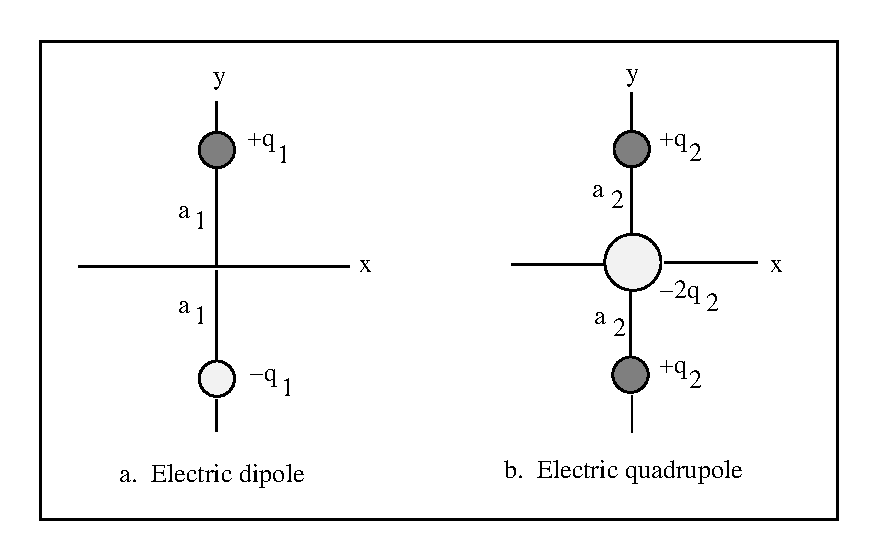
\includegraphics{charge_dist_water_mol_fig_1.eps} \par}
\vspace{0.3cm}

\textbf{Activity 1: The Electric Dipole }

(a) Calculate the electric potential, V, for the electric dipole for
a point along the y-axis, but at a position \( \left| y\right|  \)>
a\( _{1} \). Your final expression should depend on the position,
y, the charge, q\( _{1} \), and the most probable location of the
charges, a\( _{1} \).
\vspace{40mm}

(b) Generate an expression for the potential energy, U, of the charge
distribution when another charge, q\( _{test} \),  placed somewhere
on the y-axis with \( \left| y\right|  \)> a\( _{1} \).
\vspace{40mm}

(c) Recall the component of the force on a particle is related to
the potential energy of the particle by F\( _{y} \) = -\( \frac{dU}{dy} \).
Calculate the force on the test charge in terms of the position on
the y-axis, the charges, and a\( _{1} \).
\vspace{40mm}

(d) Make the approximation that the test charge is far from the molecule,
i.e., \( \left| y\right|  \) \( \gg  \) a\( _{1} \), to generate
a new expression for the force.
\vspace{40mm}

\textbf{Activity 2: The Electric Quadrupole} 

(a) Calculate the electric potential, V, for the electric quadrupole
for a point along the y-axis, but at a position \( \left| y\right|  \)
> a\( _{2} \). Your final expression should depend on the position,
y, the charge, q\( _{2} \), and the most probable location of the
charges, a\( _{2} \).
\vspace{40mm}

(b) Generate an expression for the potential energy, U, of the charge
distribution when another charge, $q_{test}$, is placed somewhere
on the y-axis with \( \left| y\right|  \) > a\( _{2} \).
\vspace{40mm}

(c) Calculate the force on the test charge in terms of the position
on the y-axis, the charges, and a\( _{2} \).
\vspace{40mm}

(d) Make the approximation that the test charge is far from the molecule,
i.e., \( \left| y\right|  \) \( \gg  \) a\( _{2} \), to generate
a new expression for the force.
\vspace{40mm}

\textbf{Activity 3: Distinguishing Between the Two Different Charge
Distributions} 

(a) Construct a table in the space below with column headings y (angstroms),
Dipole Force (arbitrary units), and Quadrupole Force (arbitrary units).
The units of distance known as angstroms are commonly used in atomic
physics. One angstrom is equal to 10\( ^{-10} \) m.
\vspace{40mm}

(b) To calculate the force on the test charge one must know the charges
and their positions for each charge distribution (q\( _{1} \), q\( _{2} \),
a\( _{1} \), a\( _{2} \)). These quantities are unknown to us at
this point. However, we want to compare the behavior of the force
due to each as a possible probe of the molecule's charge distribution.
In the expressions you generated in step (d) of Activities 1 and 2
for \( \left| y\right|  \) \( \gg  \) a\( _{1} \) or \( \left| y\right|  \)
\( \gg  \) a\( _{2} \) the forces depend on some power of y. For
\emph{convenience}, set the constant in front of this power of y to
unity. Calculate the forces for the dipole and quadrupole at distances
between 1.5 angstroms and 5.0 angstroms in 0.5 angstrom steps. Enter
your results in the table.

(c) Make a graph of the force due to the dipole and due to the quadrupole
as a function of y. Insert a copy of the graph into your notebook.

(d) In many experiments constants like those in your expressions for
the force on the test charge are unknown or poorly known. Suppose,
however, that you are able to accurately measure the radial dependence
of the force on q\( _{test} \) at distances far from the H\( _{2} \)O
molecule. If that is the case use the results from steps (b) and (c)
to propose a technique to distinguish between the two candidates for
the charge distribution of H\( _{2} \)O. Support your proposal with
a mathematical argument. (Hint: Consider a ratio involving the measured
force.)
\vspace{40mm}

(e) Experiment has found that water behaves as an electric dipole
with the electric dipole moment, q\( _{1} \)a\( _{1} \), measured
to be 6.2 x 10\( ^{-30} \) C-m. If the charge that creates the dipole,
q\( _{1} \), is the charge associated with the protons and electrons
of the molecule calculate the separation of the charges, a\( _{1} \).
How does it compare with the size of the H\( _{2} \)O molecule of
about 1.0 angstroms?\vspace{40mm}


\includelab{0}{ideal_gas_cycles/ideal_gas_cycles}
\includelab{1}{piano_tuning/piano_tuning}

%--------------------------------------------
\appendix
\setcounter{section}{4} %set this counter to number MINUS ONE corresponding to desired appendix letter. (4 for `E', etc.)
%Put include statements for supplementary appendices below here.
%                                                 
\section{Nuclear Safety}

All of the radioactive sources we will use in class are very low-level
isotopes referred to as ``license-free'' sources.
The following guidelines should be followed for handling radioactive
materials in the classroom.

%test comment by Matt
\begin{enumerate}

\item Eating, drinking, and application of cosmetics in the 
laboratory are not permitted.

\item Pipetting by mouth is never permitted. Use suction devices
such as pipette filters.

\item Gloves and lab coats should be worn when working with all liquid
isotopes.

\item Before leaving the lab, wash your hands thoroughly and check for
possible contamination with a survey instrument.

\item All radioactive liquid wastes are to be poured into the liquid
waste container, NEVER into a sink.

\item Report all spills, wounds, or other emergencies to your instructor.

\item Maintain good housekeeping at all times in the lab.

\item Store radioactive material only in the designated storage area. Do not
remove sources from the lab.

\end{enumerate}


\end{document}
